\section{Technical Writing}
\label{sec:TechnicalWriting}

One of the main powers of \LaTeX\ is the ability to format mathematics. In equation~\eqref{eqn:ClosureOfSO2} below is a simple example showing closure of the $SO(2)$ group, something that would be extremely painful to typeset in Word but is trivial to do in \LaTeX.
\begin{subequations}
\begin{align}
	R(\theta)R(\phi) &= 
	\left( \begin{array}{cc}
		\cos\theta & -\sin\theta \\
		\sin\theta & \cos\theta
	\end{array} \right)
	\left( \begin{array}{cc}
		\cos\phi & -\sin\phi \\
		\sin\phi & \cos\phi
	\end{array} \right)\label{eqn:ClosureOfSO2a}  \\
	&= \left( \begin{array}{cc}
		\cos\theta\cos\phi - \sin\theta\sin\phi & -\cos\theta\sin\phi -\sin\theta\cos\phi \\
		\sin\theta\cos\phi + \cos\theta\sin\phi & -\sin\theta\sin\phi + \cos\theta\cos\phi
	\end{array} \right)\label{eqn:ClosureOfSO2b}  \\
	&= \left( \begin{array}{cc}
		\cos(\theta + \phi) & -\sin(\theta + \phi) \\
		\sin(\theta + \phi) & \cos(\theta + \phi)
	\end{array} \right)\label{eqn:ClosureOfSO2c}  \\
	&= R(\theta + \phi)\label{eqn:ClosureOfSO2d}
\end{align}
\label{eqn:ClosureOfSO2}
\end{subequations}
We note the following that are impossible, awkward, or very manual to do in Word:

\begin{itemize}
	\item The equations are numbered automatically and we do not need to position them ourselves
	\item The equations are aligned on the equals sign - I did not need to add spaces to do this
	\item The whole equation or individual parts such as equation~\eqref{eqn:ClosureOfSO2b} can be cross-referenced easily
	\item Much more complicated configurations can be created, such as equations in two columns
\end{itemize}

Images are inserted by giving a path to the image. This means when the images are updated, the document also updates when it is recompiled. Copying by reference means there is one version of the truth which is one of the reasons why copying by value in situations like this is poor practice. I have wasted a lot of time reinserting images into documents because it appears Word only copies by value.

Word and other Microsoft Office Suite products are very poor at handling vector graphics. As an engineering consultancy, we feature many images which could be vector graphics yet are forced to rasterise, lowering their quality. The only option I have found that Word is happy with are Enhanced Metafiles (EMF), a format of Microsoft's creation with many problems\footnote{EMF files do not support transparency. They also do not or antialiasing so all text looks odd as well.}. On the other hand, \LaTeX\ handles both bitmaps and vector graphics easily.

Word's strange behaviour with images and exporting wastes time. Word will compress images for you by default when pasting an image into the document, and even stranger, the level of compression depends on how zoomed in you are. I have also seen documents where all the figures are unreadable because Word decided to compress them all between revisions. There are many ways to export to PDF in Word, all of which behave differently and compress images. \LaTeX\ will produce a PDF with the exact image it was given.

Going further than this, plots and figures can even be created inside \LaTeX\ itself, although this is typically for more advanced users. This means even the font in plot titles and axis labels can be consistent with the rest of the document and even the entire project. I have not found any other way of achieving this conveniently. Figure~\ref{fig:ExamplePlots} demonstrates the difference in quality. Even though figure~\ref{fig:ExampleRasterImage} has been well-made in Python, the lower resolution, inconsistent style, and nasty typesetting of $\pi$ symbols make it look noticibly worse than figure~\ref{fig:ExampleVectorImage}. Figure~\ref{fig:ExampleVectorImage} has infinite resolution and the added benefit of highlightable and searchable text\footnote{It is not necessary to make the figure in \LaTeX\ for this functionality, any vector image would have this.}.

\begin{figure}[H]
	\begin{subfigure}{0.49\textwidth}
		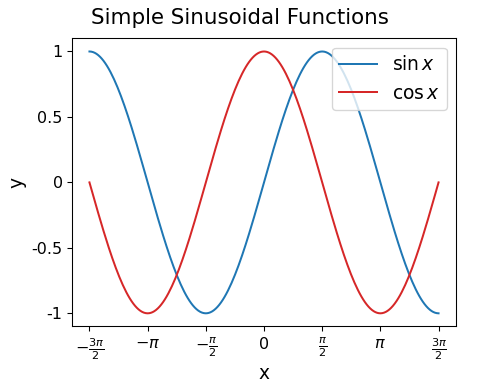
\includegraphics[width=\textwidth]{example_figure_matplotlib_096.png}
		\caption{96 dpi raster made with matplotlib}
		\label{fig:ExampleRasterImage}
	\end{subfigure}
	\begin{subfigure}{0.49\textwidth}
		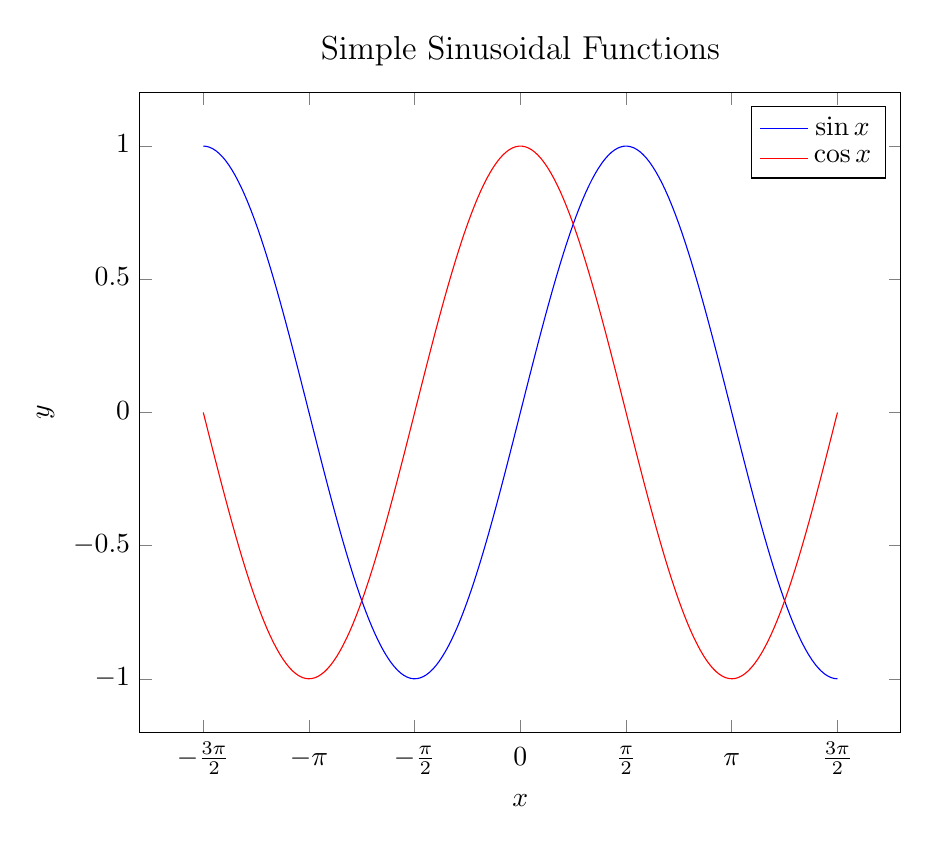
\begin{tikzpicture}
			\begin{axis}[
				height = 0.8*\textwidth,
				title = \large{Simple Sinusoidal Functions},
				xlabel = $x$,
				ylabel = $y$,
				xtick = {-1.5*pi, -pi, -pi/2, 0, pi/2, pi, 3*pi/2},
				xticklabels = {$-\frac{3\pi}{2}$, $-\pi$, $-\frac{\pi}{2}$, $0$, $\frac{\pi}{2}$, $\pi$, $\frac{3\pi}{2}$},
				typeset ticklabels with strut,
				xlabel near ticks]
				\addplot[domain = -1.5*pi:1.5*pi, samples=200, color=blue]{sin(180*x/pi)};
				\addlegendentry{$\sin x$}
				\addplot[domain = -1.5*pi:1.5*pi, samples=200, color=red]{cos(180*x/pi)};
				\addlegendentry{$\cos x$}
			\end{axis}
		\end{tikzpicture}
		\caption{Vector graphic made in \LaTeX}
		\label{fig:ExampleVectorImage}
	\end{subfigure}
	\caption{A comparison between a low quality rasterised image and a vector graphic.}
	\label{fig:ExamplePlots}
\end{figure}

Below is a list of other features of \LaTeX\ that make it better for writing technical documents that Word does not support.

\begin{itemize}
	\item Subfigures can be given automatically numbered and easily cross-referencable subcaptions.
	\item Figures and tables can be given an optional short caption which appears in the list of tables and list of figures. This means brief metadata about figures can be kept closely attached to the figures and tables in the caption without cluttering the corresponding lists.
	\item The exact positioning of objects is handled automatically. For example, the user provides the caption text and the compiler puts it in a sensible place.
	\item All formatting changes can be tracked and easily copied.
	\item Smaller file sizes and the ability to handle documents several hundred pages long easily.
	\item The output is determined exactly from the text input, so it is not possible to reload the output and get different behaviour like in Word.
\end{itemize}https://github.com/HenryGinn/Essays/tree/main/TheCaseForLaTeX

\LaTeX\ is also better for version control. As it is all text-based it can be used with version control software like Git, which gives tracability, control over branches, and easy computation of differences between versions. This also tracks any formatting changes that cannot be handled by the template such as the shape of a table.